
\chapter{Class Diagram}
\label{section:classDiagramDescription}

A class diagram is a basic UML diagram. It is probably the best known of all UML diagrams. The class diagram is used for description of system's (or program's) structure by showing its classes and their relations. 

Despite the fact that the diagram is called class diagram, it does not describe only the classes of the system. It describes all the data types like interfaces, enumeration types, etc. Concrete types (class, interface, etc.) are distinguished by stereotypes. All these data types are in the class diagram displayed as rectangles. These rectangles can be divided into three parts: 
\begin{itemize}
    \item The first part contains the name of the class (or interface, enumeration, etc.) and eventually the stereotype (a text in \guillemotleft angle quotes\guillemotright) which describes a special property (interface, enumeration, or something else). If there is no stereotype, it means that the rectangle represents a simple class.
    \item The second part contains the list of attributes. Every attribute defines its scope (public, private, protected), name and the data type. There don't have to be all the attributes in this part, but only the important ones.
    \item The last, third part, contains the list of methods. Every method defines its scope, name, list of parameters and the return value. Again, there can be only methods which are important to depict a concrete problem.
\end{itemize}

\begin{figure}[!ht]
\begin{center}
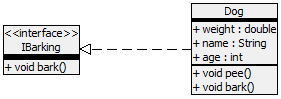
\includegraphics[]{img/classDiagramExample.png}
\caption{Example of a class diagram}
\label{f-classDiagramExample}
\end{center}
\end{figure}

Example of a class diagram (on Java platform level) can be seen in the Figure \ref{f-classDiagramExample}. There are two rectangles. First, with name IBarking, represents the interface (it has the \guillemotleft{}interface\guillemotright stereotype). This interface defines one public method with no return type (void) called bark. The second rectangle represents simple class (there is no stereotype) called Dog. The Dog class defines three public attributes (weight of the double type, name of the String type and age of the integer type) and two public methods (pee and bark), both with no return type. Between these two rectangles there is a relationship defining that the Dog class implements the IBarking interface.

As it has been already said in the last paragraph, there can be relations between classes. UML Class diagram defines 5 basic relations between classes (or interfaces and enumerations) which define some feature of the class. These relations are:

\begin{itemize}
    \item Association - this relation type defines a feature of the source class\footnote{In this chapter when I write the source or the target class, I will not mean only a class, but also an interface or an enumeration. If it is not, I will point it out.}. In the class diagram it is depicted as a solid line which leads from the source class to the target class (the target class defines the data type of the feature). The relation can also have a simple arrow defining the relation's direction. On the end of the direction (the side where the arrow is) there is the name and cardinality of the feature. You can see an association example in the Figure \ref{f-exampleAssociation}.
    \item Aggregation - defines that the target class is a part of the source class. This relation is depicted as a solid line with a blank diamond on the start (on the side where the starting/owning class is). An example of the Aggregation is shown in the Figure \ref{f-exampleAggregation}.
    \item Composition - represents stronger relation than the Aggregation. Composition tells us that when the owner object (instance of the class) is destroyed, the owned object will be destroyed as well. Composition is depicted by a solid line with a filled diamond on the start. Figure \ref{f-exampleComposition} shows an example of the Composition.
    \item Generalization - this relation defines that source class is derived from the target class. There are some restrictions for this relation. Class can be derived only from class (not from interface) and interface can be derived again only from interface. Realisation is depicted as a solid line with a solid arrow on the end. AN example of this relation can be found in the figure \ref{f-exampleGeneralization}
    \item Realisation - defines that a class (not an interface) implements an interface. Realisation is shown as a dashed line with a solid arrow on the end. The example is shown in the Figure \ref{f-exampleRealisation}
\end{itemize}

\begin{figure}[!ht]
\begin{center}
\subfigure[An Association example]{
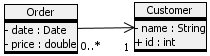
\includegraphics[scale=1]{img/exampleAssociation.png}
\label{f-exampleAssociation}
}
\subfigure[An Aggregation example]{
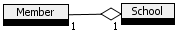
\includegraphics[scale=1]{img/exampleAggregation.png}
\label{f-exampleAggregation}
}
\subfigure[A Composition example]{
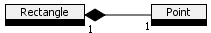
\includegraphics[scale=1]{img/exampleComposition.png}
\label{f-exampleComposition}
}
\subfigure[A Generalization example]{
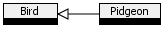
\includegraphics[scale=1]{img/exampleGeneralization.png}
\label{f-exampleGeneralization}
}
\subfigure[A Realisation example]{
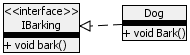
\includegraphics[scale=1]{img/exampleRealisation.png}
\label{f-exampleRealisation}
}
\caption{Relations examples}
\label{f-relationExamples}
\end{center}
\end{figure}

\section{Diagram types}

In a computer engineering, class diagram is used for both conceptual modeling (business modeling) and class modeling on platform level, which is consequently translated into a programming language (into the programming code).

Conceptual modeling is frequently used in early stage of software/system development. Its purpose is to depict the basic ideas of the domain that we want to build (a problem domain). It is why is this model often called Domain Object Model (DOM) or simply domain model. The domain model represents the vocabulary and key features of the problem domain. These features are represented by entities that occur in the problem domain, their attributes and relations between them. This type of model is really useful as a communication tool between several members of business team or between the business and technical team. By this model it can be also verified that the system meets the user's requirements, but only if this model is created well.

Class modeling on platform level describes the physical structure of the software. It uses all elements of UML class diagram, not only classes, its attributes and relations between them. More information about class diagram can be found in \cite{UMLDistilled}.

\section{Class Modeling Tools}

There are a lot of applications that provides the class modeling. Some of them can be used for free, some of them not (most of the better). This section will show several of them.

The application that inspired me most was Enterprise Architect from Sparx Systems \cite{sparxsystemsweb} company. This application does not provide only class modeling functionality. It is a CASE\footnote{CASE - Computer Aided Software/System Engineering} system which is used for purposes of analysis and implementation. The Enterprise Architect provides all UML diagrams (Class diagram, Activity diagram, Use Case diagram, Sequence diagram, etc.) creation and much more. But only the Class diagram is important for this project because it is what this thesis deals with. The class modeling in Enterprise Architect has a lot of functionality that cannot be created during a one bachelor thesis. Thus, it has to be decided which functionality will be implemented and which will not. Next list shows several applications which provides a class diagram modeling.

\begin{itemize}
    \item Enterprise Architect - Professional CASE tool for easy creation of UML diagrams and much more. More info in \cite{sparxsystemsweb}.
    \item ArgoUML - Open Source UML Modeling tool based on Java programming language. More info in \cite{ArgoUMLWeb}.
\end{itemize}
